
La soluzione al problema di discretizzazione degli stati con conseguente perdita di informazioni che potrebbe risultare importanti e decisive al learning dell'ambiente, viene risolta grazie all'algoritmo di Deep Q-network: la Q-table viene infatti sostituita da una rete neurale, la quale non necessita più di alcuna forma di discretizzazione che approssima la funzione valore.

La rete prende come input lo stato e produce una stima della funzione valore per ogni azione: in particolare si tratta di una rete \textit{fully-connected}, in cui l'imput della network sono le quattro variabili di stato
\begin{itemize}
	\item Posizione (\textit{x})
	\item Velocità lineare ($\dot{x}$)
	\item Angolo ($\theta$)
	\item Velocità angolare ($\dot{\theta}$)
\end{itemize}
mentre le uscite rappresentano i Q-values per le due possibili azioni, ovvero il movimento a destra e a sinistra, come si può vedere in figura ~\ref{fig:DQN_network}.

\begin{figure}[!h]
	\centering
	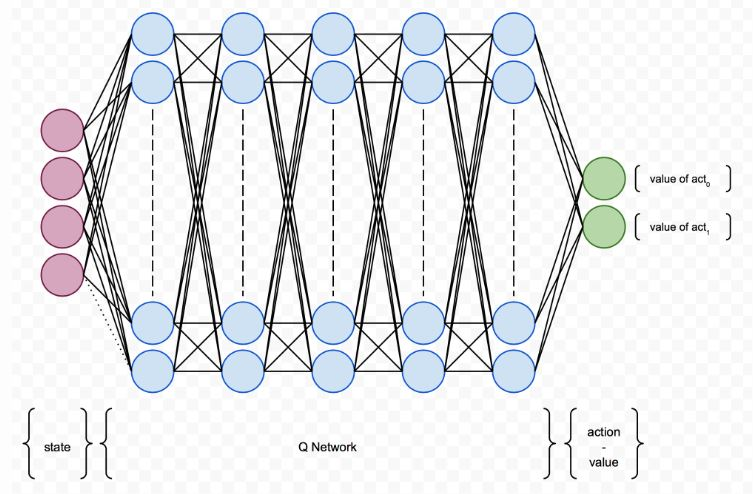
\includegraphics[width=0.7\textwidth]{Immagini/DQN_network.JPG}
	\caption{DQN network}
	\label{fig:DQN_network}
\end{figure}

\subsection{Q network}
Nell'implementazione, per andare a realizzare la rete neurale, è stata utilizzata la libreria python TensorFlow, basandosi sulle API fornite da Keras, per una facile creazione della rete neurale, in maniera molto rapida e concisa.

\begin{lstlisting}
	model = Sequential()
	model.add(Flatten(input_shape=(1,) + env.observation_space.shape))
	model.add(Dense(16))
	model.add(Activation('relu'))
	model.add(Dense(nb_actions))
	model.add(Activation('linear'))
\end{lstlisting}

Tramite l'utilizzo di una rete neurale quindi, andiamo a sostituire l'update della Q table con il train della nostra rete neurale: come infatti ben sappiamo, il modello \textit{DQN neural network} è un modello di regressione, il cui output è tipicamente un valore continuo (\textit{float value}), che rappresenta direttamente valore della nostra Q function.

L'agente, come sempre, andrà a scegliere l'azione che presenta il Q-value maggiore, che indica appunto quale è l'azione che si presume andare a dare un maggiore reward nel futuro.

\begin{figure}[!h]
	\centering
	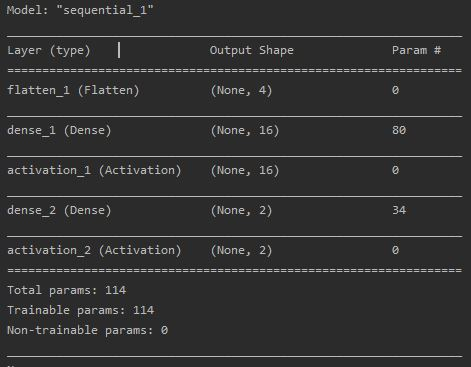
\includegraphics[width=0.5\textwidth]{Immagini/Model_of_my_net.JPG}
	\caption{Modello della rete neurale: 4 input \textit{state} e 2 output \textit{Q-action}}
	\label{fig:Model_of_DQN_network}
\end{figure} 


\subsection{Replay memory}
Introducendo una rete neurale, invece della Q-table utilizzata durante la prima versione del Q learning, la complessità del nostro ambiente può crescere significativamente, senza richiedere necessariamente più memoria: come si può facilmente vedere, un environment a celle con grandezza $50 \times 50$, andrebbe ad esaurire facilmente la memoria della maggior parte dei pc in commercio.

Invece, con una rete neurale, anche con ambienti complessi, non dobbiamo affrontare problemi legati ai requisiti di memoria.

Per gestire questo utilizzo di memoria, un concetto da illustrare è quello dell’experience replay, codificato tramite il comando presentato in figura ~\ref{fig:SeqMem}.

\begin{figure}[!h]
	\centering
	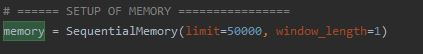
\includegraphics[width=0.5\textwidth]{Immagini/SequentialMemory.JPG}
	\caption{Creazione variabile per sequential memory}
	\label{fig:SeqMem}
\end{figure}

Gli algoritmi di reinforcement learning presentano infatti spesso il problema di avere un alto livello di correlazione tra esperienze successive con l'alto rischio di portare ad un veloce overfitting sui dati a disposizione, evitando così la necessaria generalizzazione.

L’idea della experience replay è quindi quella di salvare le esperienze
in una memoria chiamata replay memory e durante ogni passo di learning recuperare in maniera randomica un campione di tali transazioni, per andare così ad introdurre una forte incorrelazione tra misure sequenziali.

Questo è dimostrato come esso vada a stabilizzare e a migliorare la procedura di training della rete neurale DQN.

\subsection{Result}
\begin{figure}[!h]
	\centering
	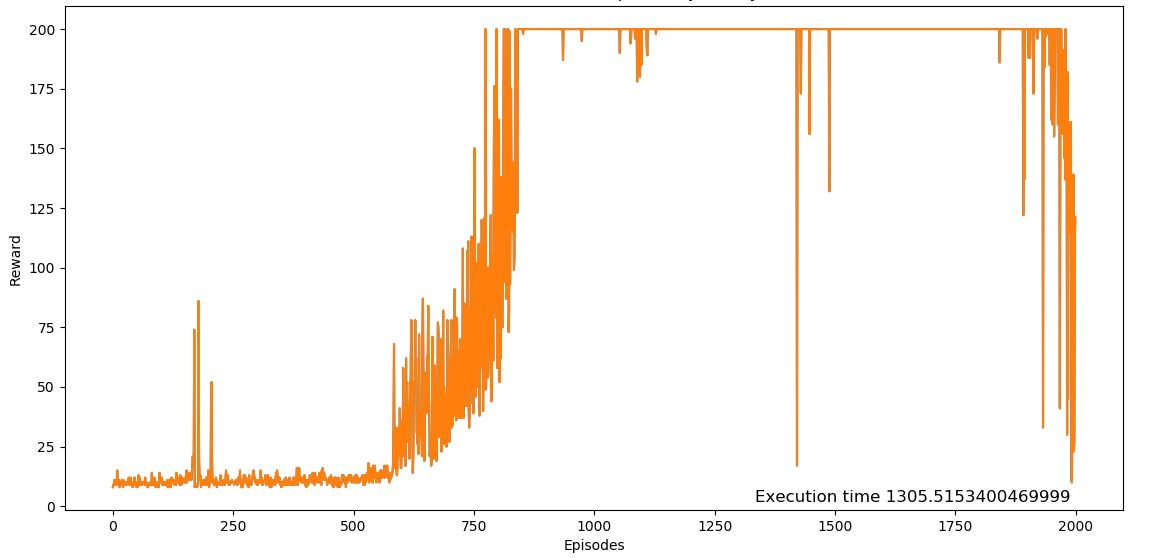
\includegraphics[width=\textwidth]{Immagini/DQN_Agent.JPG}
	\caption{Reward con DQN network}
	\label{fig:DQN_reward}
\end{figure}

\newpage